\chapter{Algorithmen}\label{ch:algorithmen}
Verschiedene Theorien/Strategien von Speicher und Ladesysteme ausarbeiten und Zeiten messen (Mit Java und JSON hauptsächlich). Verschiedene Spielarten und Speichersysteme für diese ausarbeiten (Chunk Systeme machen vielleicht nicht überall Sinn, aber allgemein Daten aufteilen müsste gut sein)

\todo{Speicher und Ladezeiten vs Speicherverbrauch Zusammenhang}
%--------------------------------------------------------------------------
%--------------------------------------------------------------------------




%--------------------------------------------------------------------------
%--------------------------------------------------------------------------
\section{Speichersysteme}\label{sect:speichersysteme}
Dieser Abschnitt befasst sich ausführlich mit dem komplexen Speicherprozess eines Videospieles. Dabei wird zunächst eine gründliche Analyse der Struktur eines Spiels durchgeführt, um zu verstehen, wie es aufgebaut ist und welche vielfältigen Datentypen verwendet werden. Anschließend werden verschiedene fortschrittliche Strategien und wichtige Faktoren im Zusammenhang mit dem Speichersystem eines Spiels detailliert vorgestellt.
%--------------------------------------------------------------------------


%--------------------------------------------------------------------------
\subsection{Daten in Videospielen}
Um sich weiter mit Speicher- und Ladesystemen auseinanderzusetzen, muss erst einmal definiert werden, welche Arten von Daten es in Videospielen gibt. Allgemein können die Daten in zwei Kategorien unterteilt werden. Ein Videospiel hat \textit{statische} und \textit{dynamische} Daten.

\textit{Statische Daten} sind, wie der Name es schon sagt, Daten, die sich nicht mehr verändern. Statische Daten eines Spieles können zum Beispiel die ganzen Grafikdaten und audiotechnischen Daten sein. Spiele haben fast immer Charaktere, Texturen, Musik oder Soundeffekte, die einmal erstellt werden und danach unverändert im Spiel geladen werden. Bei vielen Videospielen gibt es auch Level- oder Kartendaten. Wenn diese sich nie während des Spieles verändern und fest definiert sind, sind diese ebenfalls eine Art von statischen Spieldaten. \todo{Updaten von statischen Daten erwähnen (Paper einbeziehen)}

\textit{Dynamische Daten} dagegen sind auch wie es der Name verrät Daten, die sich ständig verändern können. Hierbei handelt es sich oft um den Spielstand eines erstellten Spieles. Dazu gehören dann zum Beispiel die Position des Spielers, seine Rotation, seine aktuelle Geschwindigkeit oder sein Inventar. Alles Daten, die sich andauernd während des Spielens verändern können. Zu den dynamischen Daten können auch Benutzerdaten gehören. Bei einigen Spielen wird ein Benutzername mit Passwort und Avatar benötigt. Dies sind auch Daten, die sich gelegentlich verändern können.

Der Fokus dieser Arbeit liegt bei dynamischen Daten, genauer gesagt, wie der Spielstand eines Spieles effizient gespeichert und geladen werden kann. Für dynamische Daten gibt es viel mehr Speicherprozesse während der Laufzeit des Videospiels, was das effiziente Speichern herausfordernder macht. Da Benutzerdaten recht selten sich verändern, stehen diese auch nicht im Schwerpunkt der Arbeit.  
%--------------------------------------------------------------------------


%--------------------------------------------------------------------------
\subsection{Spielphasen} \label{ssect:spielphasen}
Um zu verstehen, wann ein Spielstand gespeichert oder geladen werden muss, muss erst einmal analysiert werden, welche Phasen ein Videospiel allgemein hat.

\begin{figure}[htp]
    \centering
    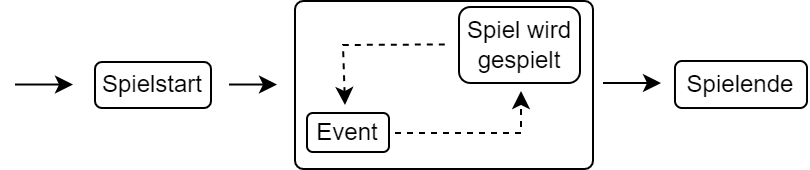
\includegraphics[width=0.8\textwidth]{images/Spielphasen.png}
    \caption{Phasen eines Spieles}
    \label{fig:spielphasen}
\end{figure}

In der Abbildung \ref{fig:spielphasen} ist zu erkennen, wie der Ablauf einer generellen Spielphase in Videospielen gestaltet ist. Der Prozess beginnt mit dem Spielstart, bei dem der Benutzer die Wahl zwischen dem Erstellen eines neuen Spiels oder dem Laden eines bereits vorhandenen Spielstands treffen muss. Sobald diese Eröffnungsphase abgeschlossen ist, wird die Hauptphase erreicht. Die Dauer dieser Phase hängt von der Spieldauer ab, da hier der Benutzer aktiv ins Geschehen eingreift und das Videospiel spielt.

In dieser Spielphase können vielfältige Ereignisse auftreten, die entweder direkt oder indirekt als Reaktion auf die Aktionen des Spielers entstehen. Die Ereignisse äußern sich in Form von Veränderungen an Spielobjekten, entweder durch Modifikation, Hinzufügung oder Löschung dieser. Beispielsweise kann der Spieler in eine neue Region vorstoßen, wodurch Daten dieser Region geladen und möglicherweise Daten der vorherigen Region gespeichert werden müssen. Das Spielobjekt des eigenen Charakters wurde in diesem Fall verändert, denn es wurde zum Beispiel die Position und Region des Spielers verändert. Vielleicht müssen dann auch neue Gegner erstellt oder stehen gelassene Items der alten Region gelöscht werden. 

Sobald der Spieler sich dazu entscheidet, das Spiel zu beenden, gelangt er zur Phase des Spielendes. Hierbei ist es eventuell erforderlich, Daten zu speichern, bevor das Programm ordnungsgemäß beendet werden kann oder die Rückkehr zum Hauptbildschirm des Spiels erfolgt. Diese Phase des Spielendes markiert einen Schlusspunkt in der aktuellen Spielsitzung. Wenn diese wieder fortgesetzt werden soll, muss der Spielstand, der bei dem letzten Beenden des Spieles erreicht wurde, wieder vollständig hergestellt werden. 
%--------------------------------------------------------------------------


%--------------------------------------------------------------------------
\subsection{Delta-basierte Speicherung} \label{ssect:deltasave}
Um die Menge der zu speichernden Daten zu reduzieren, empfiehlt es sich, auf eine delta-basierte Speicherung zurückzugreifen. Bei dieser Methode werden lediglich die Daten gespeichert, die sich seit dem letzten Speichervorgang verändert haben. Insbesondere bei großen Datenmengen entfaltet diese Speichertechnik ihre volle Effektivität, da dann oft nur ein geringer Prozentsatz der Gesamtdatenmenge tatsächlich abgespeichert werden muss und somit der Speicherbedarf stark reduziert wird. Um stets den Überblick darüber zu behalten, welche Veränderungen eingetreten sind, gilt es, auf Ereignisse zu achten, bei denen Modifikationen, Hinzufügungen oder Löschungen von Spielobjekten auftreten.

Um die Anzahl der Lese- und Schreibprozesse möglichst stark zu minimieren, kann eine Datei erstellt werden, in der zur Laufzeit des Spieles eine Liste aller Veränderungen der Spielobjekte geführt wird. Hierbei muss nicht das ganze Objekt gespeichert werden, es reicht, die Identifikationsnummer des Objekts und die veränderten Attribute zu speichern. Somit sind die jeweiligen Schreibprozesse auf dem lokalen Speicher deutlich kleiner während der Laufzeit. Wenn die Spielwelt wieder gestartet und geladen wird, können diese Veränderungen dann endgültig bei den gespeicherten Spielobjekten angewandt werden, um diese zu aktualisieren. Danach kann diese Liste von Veränderungen wieder geleert werden und das Spiel kann gestartet werden.
%--------------------------------------------------------------------------


%--------------------------------------------------------------------------
\subsection{Aufteilung der Daten} 
Eine weitere Art, die Datenmenge besser zu organisieren, um dann Speicherprozesse zu reduzieren, ist das Aufteilen der Daten. Wenn die ganze Datenmenge in sinnvolle Gruppen unterteilt wurde, ist es nicht notwendig, jedes Mal die ganze Datenmenge zu durchlaufen. Stattdessen kann sich immer nur eine bestimmte Gruppe vorgenommen werden. In diesem Abschnitt werden zwei Möglichkeit der Aufteilung der Spieldaten betrachtet, einmal mit Chunks und einmal nach Level oder Karten der Spielwelt. Beide Strategien haben unterschiedliche Szenarien, wann es sinnvoll ist, diese einzusetzen.

\subsubsection{Chunks} \label{sssect:chunks}
Eine sehr weit verbreitete Art der Aufteilung von Spieldaten sind \textit{Chunks}. Chunks haben bei Videospielen meist eine feste Position und sind alle gleich groß. Daten werden dann abhängig von deren Position zu dem entsprechenden Chunk zugeteilt. Vorteilhaft an dieser Herangehensweise ist, dass recht einfach und schnell gefiltert werden kann, welche Daten bei dem aktuellen Spielstand relevant sind. Beim Speichern und Laden können dann nur Chunks in der Nähe des Spielers betrachtet werden. Außerdem können Spielwelten mit dieser Struktur theoretisch unendlich sein, die Größe muss nicht festgesetzt sein. Es gibt auch Variationen von Chunk-Systemen. Es kann zum Beispiel entschieden werden, ob ein \textit{statisches} oder \textit{dynamisches Chunk-System} verwendet werden soll. Bei einem \textit{statischen Chunk-System} wird die Chunkgröße fest auf einen Wert definiert und wird sich auch nie verändern. Bei einem \textit{dynamischen Chunk-System} passen sich die Chunkgrößen an, je nach Menge der Daten in einem Chunk. Wenn zu viele Daten in einem Chunk sind, werden weitere Chunks erstellt, um die Daten des ursprünglichen Chunks auf diese aufzuteilen. Die Abbildung \ref{fig:chunkSplitting} zeigt ein Beispielszenario, wo in einem Chunk zu viele Charaktere sind und dieser dann in vier gleich große Chunks aufgeteilt wird. Wenn zu wenig Daten in einem Chunk sind, dann werden benachbarte Chunks wieder vereinigt, um sich die Daten zu teilen. Die Abbildung \ref{fig:chunkJoining} demonstriert den Fall, dass vier benachbarte Chunks zu wenig Inhalt haben und deshalb zu einem einzelnen Chunk vereint werden. Diese Variation des Chunk-Systems ist gerade dann sinnvoll, wenn sich die Datenmenge stetig und stark verändern kann. 
\todo{Mehr Quellen, aus Google Scholar}

\begin{figure}[htp]
    \centering
    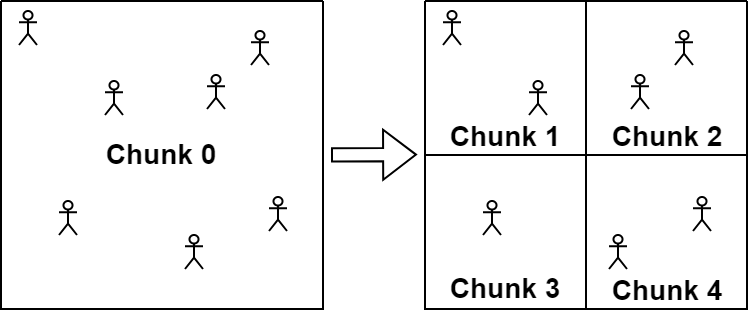
\includegraphics[width=0.6\textwidth]{images/chunkSplitting.png}
    \caption{Vollen Chunk auf kleinere aufteilen}
    \label{fig:chunkSplitting}
\end{figure}

\begin{figure}[htp]
    \centering
    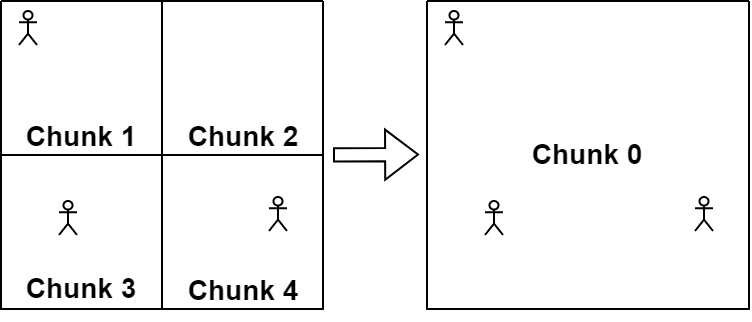
\includegraphics[width=0.6\textwidth]{images/chunkJoining.png}
    \caption{Leere Chunks vereinigen}
    \label{fig:chunkJoining}
\end{figure}

Allgemein sind Chunk-Systeme hilfreich, wenn die Spielwelt theoretisch unendlich ist. Außerdem sind sie eine recht einfache und effiziente Art, Daten klar voneinander zu trennen und zu gruppieren. Chunks haben eine quadratische oder bei dreidimensionalen Spielen kubische Form. Deutlich aufwendiger wäre es, mit anderen Formen wie Polygonen die Welt aufzuteilen. Dann zu schauen, welches Spielobjekt in welchem Chunk ist, würde mehr und kompliziertere Berechnungen benötigen. Ein dynamisches Chunk-System wäre auch nur sinnvoll, wenn in einem Chunk theoretisch unendlich viele Spielobjekte existieren können. Wenn das Spiel keine Grenze hat für Spielobjekte pro Chunk, dann ist es auch schwierig vorherzusehen, wie groß die Chunks sein müssen, sodass es nicht zu Problemen in der Leistung des Spieles kommt. 

\subsubsection{Level oder Karten}
Wenn die Spielwelt aus statischen Elementen wie Level oder Karten besteht, dann können die Daten auch nach Szenen oder Räumen aufgeteilt werden. Es können dann immer nur die Szenen oder Räume gespeichert oder geladen werden, in denen der Spieler sich momentan befindet. Falls die Szenen oder Räume zu groß werden, können diese auch in Sektoren oder Chunks aufgeteilt werden, damit nicht zu viele Daten durchlaufen werden müssen.    
%--------------------------------------------------------------------------


%--------------------------------------------------------------------------
\subsection{Serialisieren}
%\url{https://en.wikipedia.org/wiki/Comparison_of_data-serialization_formats}

\textit{Serialisierung} ist der Prozess, bei dem ein Objekt zu einer Ansammlungen von Bytes umgewandelt wird oder der Zustand eines Objekts in ein Medium abgespeichert wird, um es später wiederherzustellen oder zu übertragen, wobei die Datenstruktur und der Inhalt des Objekts in einer für die Speicherung oder Übertragung geeigneten Form kodiert werden. \textit{Deserialisierung} ist der Gegenprozess von Serialisierung, der den zuvor serialisierten Zustand wieder in das ursprüngliche Objektformat zurückführt, indem die kodierten Daten aus dem Medium extrahiert werden, die ursprüngliche Datenstruktur rekonstruiert und folglich das Objekt in seinen initialen Zustand zurückversetzt.\cite{codeguruWorkingWith}

Es gibt verschiedene Herangehensweisen, um Daten zu Serialisieren. In diesem Abschnitt werden einige Strategien genauer betrachtet. Als erstes wird die populäre Serialisierung mit \ac{json} und der binären Version mit \ac{bson} angeschaut. Zum Schluss wird die kompakte binäre Serialisierung betrachtet und wie diese umgesetzt werden kann.

\subsubsection{JSON}
Eine sehr beliebte Möglichkeit, Objekte auf Medien abzuspeichern, ist im \textit{\ac{json}-Format}. \ac{json} ist eine Kodierung von Daten, die für Menschen lesbar ist und wurde Anfang der 2000er Jahre erfunden. \ac{json}-Objekte sind Ansammlungen von Werten, denen jeweils ein Schlüssel in der Form eines String-Wertes zugeordnet wird. Unterstützte Datentypen sind String, Boolean, Number, Array, Object und null. \ac{json} wird häufig für APIs, Konfigurations-Dateien und als Datenbank-Speicher verwendet. Aber es kann auch dazu verwendet werden, dass der Zustand eines Objektes in lokalen Dateien abgespeichert wird.\cite{mongodbJSONBSON} 
In dem Code aus \ref{lst:jsonExp} ist zu sehen, wie ein Objekt im \ac{json}-Format abgespeichert werden kann. Das entsprechende Klassendiagramm des zu speichernden Objektes ist in der Abbildung \ref{fig:monsterBspKlasse} zu sehen. Das Objekt "position" besteht aus den Variablen x und y, die den Typ Number speichern, und das "effects" Array ist ein String-Array. 

\begin{listing}[htp]
    \begin{minted}{javascript}
        {
            "id": 1,
            "name": "Vampir",
            "position": {
                "x": 0.15,
                "y": 2.34
            },
            "effects": [
                "giftig", 
                "frost"
            ]
        }
    \end{minted}
    \caption{Beispiel für ein \ac{json}-Objekt}
    \label{lst:jsonExp}
\end{listing}

\begin{figure}[htp]
    \centering
    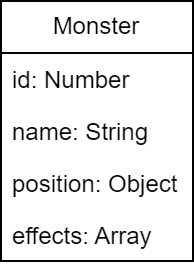
\includegraphics[width=0.18\textwidth]{images/MonsterBspKlasse.png}
    \caption{Klassendiagramm des Beispiel \ac{json}-Objektes aus \ref{lst:jsonExp}}
    \label{fig:monsterBspKlasse}
\end{figure}

Wenn sich für \ac{json} entschieden wurde, gibt es drei Arten, die Daten zu verarbeiten. Die erste ist mit einer \textit{Streaming API}, mit der man direkt \ac{json}-Objekte mit Schlüsseln und Werten erstellen kann oder direkt auf Schlüsselwerte von \ac{json}-Objekten zugreifen kann über den  entsprechenden Schlüssel. In dem Pseudocode \ref{lst:streamingApiBsp} ist zu sehen, wie mit einer Streaming API das \ac{json}-Objekt aus \ref{lst:jsonExp} erstellt werden kann. Die letzten drei Zeilen sollen einen Zugriff auf Werte des \ac{json}-Objektes darstellen.\cite{tutorialspointJacksonStreaming} Das \textit{Tree Model} dagegen arbeitet mit einem \ac{json}-Dokument, welches in dem Arbeitsspeicher als Baumstruktur gespeichert wird, wodurch das Aktualisieren von Daten sehr schnell abläuft. Diese Baumstruktur kann dann als \ac{json}-String in einer lokalen Datei abgespeichert werden. Zuletzt gibt es noch das \textit{Data Binding}, welches die Objekte direkt zu \ac{json} serialisiert und umgekehrt deserialisiert. In dem Pseudocode \ref{lst:dataBindingBsp} ist zu sehen, wie ein neu erstelltes Objekt direkt als \ac{json}-Objekt in einer Datei gespeichert wird. Das Objekt ist aus der Monster-Klasse der Abbildung \ref{fig:monsterBspKlasse}. Danach wird das Objekt mit den Werten eines \ac{json}-Objektes einer anderen Datei gesetzt.\cite{tutorialspointJacksonData}\cite{tutorialspointJacksonOverview}

\begin{listing}[htp]
    \begin{minted}{java} 
        writeStartObject()
        writeField("id", 1)
        writeField("name", "Vampir")
        writeField("name", "Vampir")
        writeFieldName("position")
        writeStartObject()
        writeField("x",  0.15) 
        writeField("y",  2.34) 
        writeEndObject()
        writeFieldName("effects")
        writeStartArray()
        write("giftig") 
        write("frost")
        writeEndArray()

        get("id")
        get("position").get("x")
        get("effects")[0]
    \end{minted}
    \caption{Psuedocode Beispiel für eine Streaming API}
    \label{lst:streamingApiBsp}
\end{listing}

\begin{listing}[htp]
    \begin{minted}{java} 
        Monster monster = new Monster()
        monster.setID(1)
        monster.setName("Vampir")
        monster.setPosition(new Position(0.15, 2.34))
        monster.setEffects(new String[]{"giftig", "frost"})
        toJSON("data1.json", monster)

        monster = toObject("data2.json")
    \end{minted}
    \caption{Psuedocode Beispiel für Data Binding}
    \label{lst:dataBindingBsp}
\end{listing}

\subsubsection{BSON}
\textit{\ac{bson}} ist eine binäre Kodierung von \ac{json}-Daten und wurde für die NoSQL-Datenbank MongoDB entwickelt. Es ist mit BSON möglich, jede \ac{json}-Dokumente zu speichern. BSON unterstützt alle Datentypen von \ac{json} und erweitert diese noch mit weiteren Typen, wie einem Datum-Typ und ein BinData-Typ. Außerdem wird mit Zahlen anders gearbeitet. Während \ac{json} Zahlen als Zeichenketten speichert, werden diese bei BSON als 32- oder 64-Bit Integers oder 64-Bit Gleitkommazahl gespeichert. Was BSON auch noch zusätzlich einführt, ist eine maximale Dokumenten-Größe von 16 MB. BSON hat gegenüber \ac{json} den Vorteil, dass die Daten viel schneller durchlaufen werden können, indem viele Datentypen mit einer festen Länge und bei Datentypen mit variabler Länge die Information der Länge gespeichert werden. Ein großer Nachteil von BSON ist, dass durch die binäre Kodierung die Lesbarkeit wegfällt.\cite{bsonspecBSONBinary}\cite{postgreSQLandBSON}\cite{mongodbJSONBSON}

Das \ac{json}-Dokument aus \ref{lst:bsonJsonObj} wäre äquivalent zu dem BSON-Dokument aus \ref{lst:bsonExp}. Die erste Zeile von dem BSON-Dokument beschreibt immer die Größe des ganzen Dokuments. In der nächsten Zeile definiert, dass es sich bei der ersten Variable des Dokuments um einen String-Typen handelt. Jeder Typ hat eine eigene Kodierung, um diesen zu identifizieren, wobei String als 0x02 kodiert wird. Die nächsten zwei Zeilen definieren den Schlüssel und Schlüsselwert des Strings. Mit 0x00 wird das Ende des Dokuments gesetzt, wie in der letzten Zeile zu sehen ist.

\begin{listing}[htp]
    \begin{minted}{javascript}
        {"hello": "world"}
    \end{minted}
    \caption{Weiteres Beispiel eines \ac{json}-Dokuments \cite{mongodbJSONBSON}}
    \label{lst:bsonJsonObj}
\end{listing} 

\begin{listing}[htp]
    \begin{minted}{javascript} 
        \x16\x00\x00\x00           
        \x02                      
        hello\x00                  
        \x06\x00\x00\x00world\x00  
        \x00                       
    \end{minted}
    \caption{BSON Kodierung des \ac{json}-Dokuments aus \ref{lst:bsonJsonObj} \cite{mongodbJSONBSON}}
    \label{lst:bsonExp}
\end{listing}

\subsubsection{Binäre Serialisierung} \label{sssec:binSerialisierung}
Bei der \textit{binären Serialisierung} wird ein Objekt als Menge von Bytes konvertiert, um es anschließend zu speichern oder über das Netzwerk zu übertragen. Während dieses Vorgangs wird jede Variable eines Objekts in eine binäre Darstellung umgewandelt, die vom Datentyp der jeweiligen Variable abhängt. Die Entscheidung für die Verwendung binärer Serialisierung ist vorteilhaft, wenn höchste Priorität auf Leistung und Kompaktheit der gespeicherten Daten gelegt wird. Jedoch hat die Leistung seinen Preis, denn das Ergebnis der Serialisierung ist nicht für Menschen lesbar. Zudem können Änderungen an dem zu serialisierenden Objekt, wie beispielsweise das Hinzufügen oder Löschen von Variablen, dazu führen, dass ältere binäre Daten nicht mehr erfolgreich deserialisiert werden können.\cite{microsoftBinarySerialization}\cite{programmathicallyUnderstandingBinary}

Eine populäre Umsetzung der binären Serialisierung ist der \textit{Protocol Buffer}. Dieser wurde Anfang 2001 von Google entwickelt und wird seitdem in vielen Projekten von Google, anderen Unternehmen und Entwicklern verwendet. Der\todo{Der?} Protocol Buffer verwendet kompilierte Daten, um diese zu binären Daten zu serialisieren. Das besondere dabei ist, dass der Protocol Buffer in verschiedenen Programmiersprachen und Plattformen verwendet werden kann. Es ist also möglich, dass die Programmierumgebung beim Serialisieren ganz anders ist, als die beim Deserialisieren. Da es sich um eine binäre Serialisierung handelt, sind die Daten zwar nicht für Menschen leserlich, jedoch ist Protocol Buffer eine schnelle und kompakte Art, Daten zu serialisieren. Bei den Abbildungen \ref{fig:protobufTime} und \ref{fig:protobufBrowser} ist zu sehen, wie schnell der Protocol Buffer im Vergleich zu JSON-Serialisierung ist.  In der Abbildung \ref{fig:protobufBrowser} ist auch zu sehen, dass die Protocol Buffer-Daten kompakter als die JSON-Daten sind. Welchen Vorteil dies auf die Effizienz anbieten wird, wird in dem Abschnitt \ref{ssec:kompression} diskutiert.\cite{currier2022protocol}

\begin{figure}[htp]
    \centering
    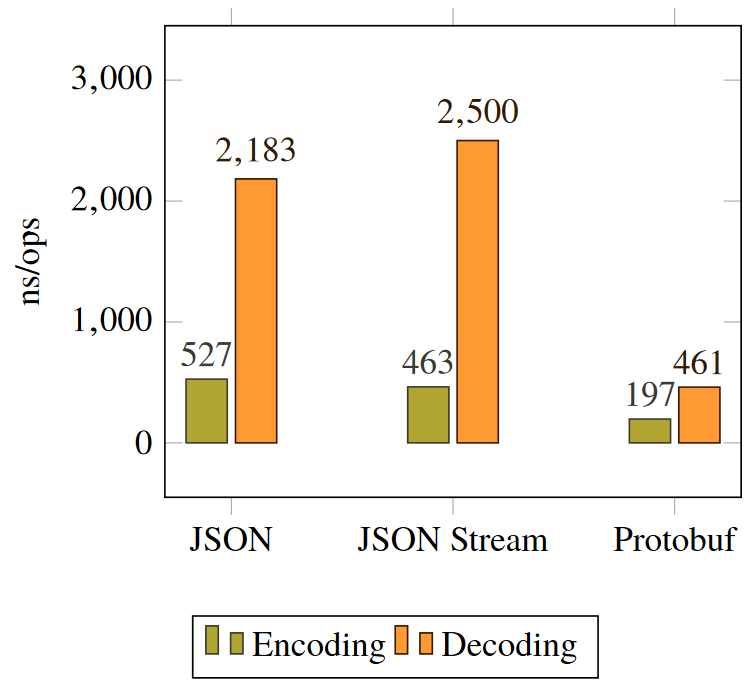
\includegraphics[width=0.7\textwidth]{images/protobuf_time.png}
    \caption{Kodierungs- und Dekodierungszeiten im Vergleich\cite{currier2022protocol}}
    \label{fig:protobufTime}
\end{figure}

\begin{figure}[htp]
    \centering
    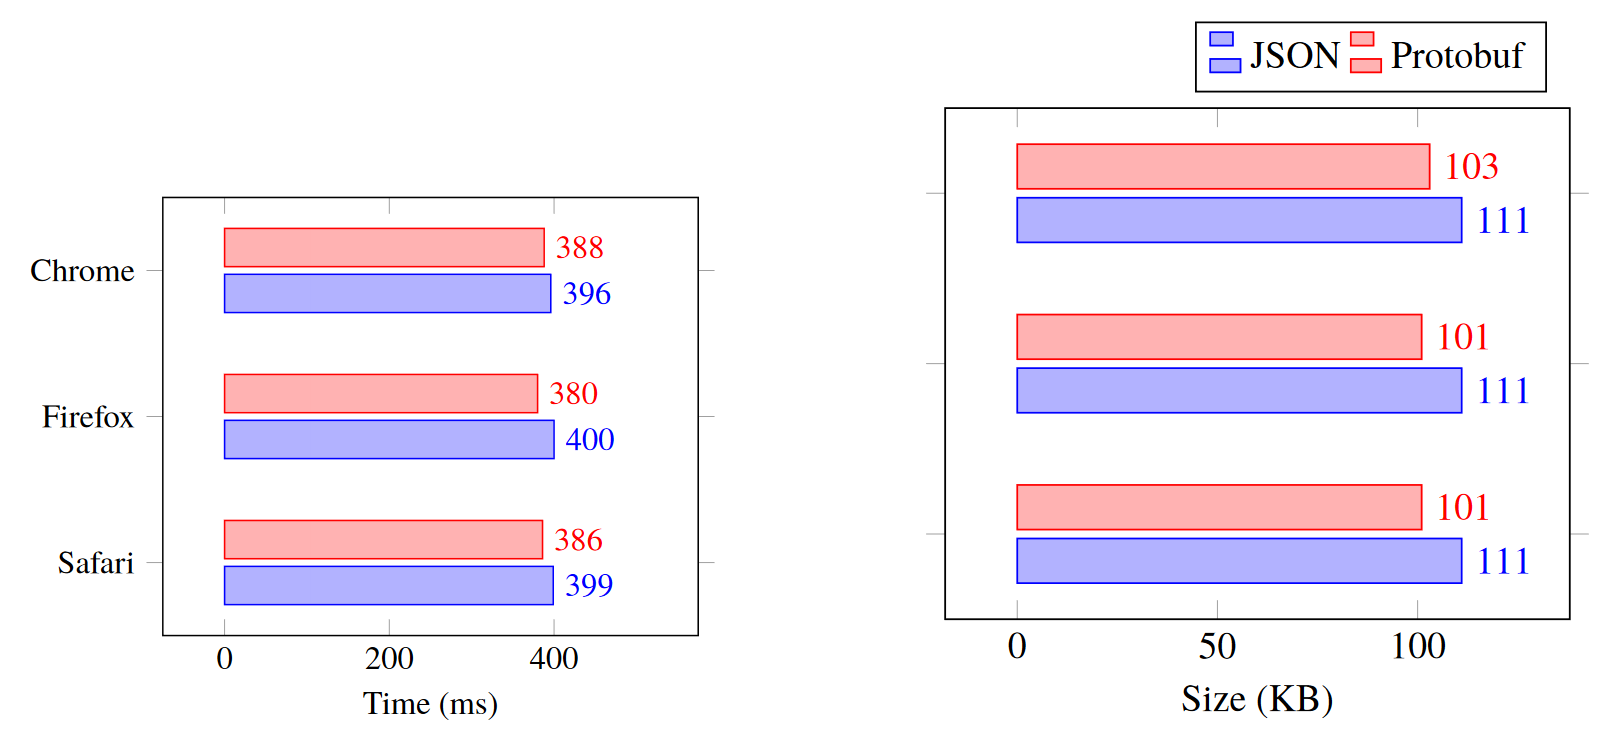
\includegraphics[width=1\textwidth]{images/protobuf_browser.png}
    \caption{Laufzeit- und Datengrößen-Vergleich\cite{currier2022protocol}}
    \label{fig:protobufBrowser}
\end{figure}

Um mit Protocol Buffer zu arbeiten, muss als erstes eine ".proto"-Datei erstellt werden. Diese Datei definiert die Datenstrukturen, die von dem Programm gespeichert werden sollen. Der Code \ref{lst:protoExp} zeigt, wie so eine Proto-Datei aussehen kann. Dabei wurde die Klasse aus der Abbildung \ref{fig:monsterBspKlasse} als Protocol Buffer-Klasse geschrieben. In so einer Proto-Datei muss immer in der ersten Zeile definiert werden, mit welcher Protocol Buffer-Version gearbeitet wird. In dem Beispiel aus \ref{lst:protoExp} wird mit der dritten Protocol Buffer-Version gearbeitet, welche aktuell die neuste Version ist. In einer Proto-Datei werden verschiedene Datentypen unterstützt. Mit der "message" können neue Datenstrukturen definiert werden. Die Klasse Monster zum Beispiel besteht aus einer nicht-negativen 32-Bit Integer Identifikationsnummer, einem String der den Namen beschreibt, eine Position und eine Liste von Effekten. Die Position wird dabei als neue Klasse in der Monster-Klasse definiert und besteht aus den Gleitkommazahlen x und y. Falls nur bestimmte Werte für eine Variable gesetzt werden sollen, kann das Enum verwendet werden. In dem Beispiel aus \ref{lst:protoExp} wird das Enum für die verschiedenen Effekte, die ein Monster haben kann, verwendet. Durch die "repeated"-Annotation wird hier eine Liste von Effekten definiert.\cite{protobufLanguageGuide}\cite{protobufProtocolBufferJava}

\begin{listing}[htp]
    \begin{minted}{cpp} 
        syntax = "proto3";
        
        message Monster {
            uint32 id = 1;
            string name = 2;

            message Position {
                float x = 1;
                float y = 2;
            }

            Position position = 3;

            enum Effect {
                GIFTIG = 0;
                PARALYSE = 1;
                FROST = 2;
                ...
            }

            repeated Effect effects = 4;
        }
    \end{minted}
    \caption{Proto-Datei einer Monster-Klasse}
    \label{lst:protoExp}
\end{listing}

Anschließend kann mit dem \ac{protoc} die Proto-Datei kompiliert werden, um die Datenstrukturen in eine gewünschte Programmiersprache zu erstellen. In der Abbildung \ref{lst:protocJava} ist zu sehen, wie der \ac{protoc}-Befehl aussehen würde, wenn mit der Java-Programmiersprache gearbeitet werden würde. Dabei müssen drei Pfade angegeben werden. Als erstes den Pfad, wo sich der Quellcode der Anwendung befindet, dann der Pfad, in der die generierten Datenstrukturen gespeichert werden sollen und zum Schluss den Pfad zu der erstellten Proto-Datei. Statt Java kann \ac{protoc} seit der dritten Version die Datenstrukturen auch in C++, Kotlin, Python, Go, Ruby, Objective-C, C\# und PHP generieren lassen.\cite{protobufLanguageGuide}\cite{protobufProtocolBufferJava}

\begin{listing}[htp]
    \begin{minted}{java} 
        protoc -I=<Pfad 1> --java_out=<Pfad 2> <Pfad 3>/data.proto
    \end{minted}
    \caption{Protoc Kommandozeilenbefehl für Java\cite{protobufProtocolBufferJava}}
    \label{lst:protocJava}
\end{listing}

Bei den generierten Datenstrukturen wird für jede Message eine Klasse erstellt. Jede Klasse hat seine eigene Builder-Klasse, um Instanzen dieser Klasse generieren lassen zu können. Die erstellten Klassen haben alle automatisch generierte Funktionen und Variablen, abhängig von den Variablen der Messages. In dem Code aus \ref{lst:protoJavaGeneratedMonster} und \ref{lst:protoJavaGeneratedBuilder} ist zu sehen, welche Funktionen die generierten Klassen haben, die aus der Monster-Message aus \ref{lst:protoExp} resultieren würden. 

\begin{listing}[htp]
    \begin{minted}{java} 
        // required uint32 id = 1;
        public boolean hasId();
        public int getId();

        // required string name = 2;
        public boolean hasName();
        public String getName();

        // required Monster.Position position = 3;
        public boolean hasPosition();
        public Position getPosition();

        // repeated Monster.Effect effects = 4;
        public List<Effect> getEffectsList();
        public int getEffectsCount();
        public Effect getEffects(int index);
    \end{minted}
    \caption{Generierte Monster-Klasse aus der Monster Message}
    \label{lst:protoJavaGeneratedMonster}
\end{listing}

\begin{listing}[htp]
    \begin{minted}{java} 
        // required uint32 id = 1;
        public boolean hasId();
        public int getId();
        public Builder setId(int value);
        public Builder clearId();

        // required string name = 2;
        public boolean hasName();
        public String getName();
        public Builder setName(String value);
        public Builder clearName();

        // required Monster.Position position = 3;
        public boolean hasPosition();
        public Position getPosition();
        public Builder setPosition(Position value);
        public Builder clearPosition();

        // repeated Monster.Effect effects = 4;
        public List<Effect> getEffectsList();
        public int getEffectsCount();
        public Effect getEffects(int index);
        public Builder setEffects(int index, Effect value);
        public Builder addEffects(Effect value);
        public Builder addAllEffects(Iterable<Effect> value);
        public Builder clearEffects();
    \end{minted}
    \caption{Generierte Builder-Klasse für die Monster-Klasse}
    \label{lst:protoJavaGeneratedBuilder}
\end{listing}

In den Code-Ausschnitten \ref{lst:protobufJavaWrite} und \ref{lst:protobufJavaRead} ist zu sehen, wie letztendlich in Java die Daten in einer Datei binär gespeichert und geladen werden können. Dafür wird hauptsächlich mit den generierten Buildern gearbeitet, denn diese können mit der Funktion "build" eine neue Monster-Instanz mit den gespeicherten Werten erstellen und mit "writeTo" diese Instanz serialisieren, um sie dann in eine gegebene Datei zu schreiben. Mit der Funktion "parseFrom" der Monster-Klasse wird eine neue Instanz aus einer Datei geladen. 

\begin{listing}[htp]
    \begin{minted}{java} 
        Monster.Builder monster = Monster.newBuilder();
        monster.setId(1);
        monster.setName("Vampir");

        Monster.Position.Builder position = Monster.Position.newBuilder();
        position.setX(0.15f);
        position.setY(2.34f);
        monster.setPosition(position.build());

        monster.addEffects(Monster.Effect.GIFTIG);
        monster.addEffects(Monster.Effect.FROST);

        FileOutputStream output = new FileOutputStream("filename");
        monster.build().writeTo(output);
        output.close();
    \end{minted}
    \caption{Schreiben von Daten mit den Protocol Buffer-Klassen in Java}
    \label{lst:protobufJavaWrite}
\end{listing}

\begin{listing}[htp]
    \begin{minted}{java} 
        Monster monster = Monster.parseFrom(new FileInputStream("filename"));
    \end{minted}
    \caption{Lesen von Daten mit den Protocol Buffer-Klassen in Java}
    \label{lst:protobufJavaRead}
\end{listing}

\todo{XML und andere Alternativen aufzählen? Kleines Fazit?}
%--------------------------------------------------------------------------


%--------------------------------------------------------------------------
\subsection{Datenkompression} \label{ssec:kompression}
Kompression von Daten ist bei vielen Software-Projekten weit verbreitet, um die Menge der gespeicherten Daten zu reduzieren. Da es bei diesem Paper aber um Laufzeit-Effizienz und nicht um eine effiziente und kompakte Nutzung des Speicherplatzes geht, stellt sich erst einmal die Frage, ob Datenkompression für das Speichern der Daten von Videospielen überhaupt notwendig ist. Datenkompression ist ein zeitintensiver Prozess. Lohnt es sich dann, Datenkompression zum Speichern des Spielstandes anzuwenden? 

Um diese Frage zu beantworten, muss erst mal geschaut werden, wann und wo Datenkomprimierung verwendet wird. Hauptsächlich wird Datenkompression verwendet, wenn eine große Datenmenge gespeichert werden muss. Je nach Algorithmus ist es durchaus möglich, dass die komprimierte Datenmenge weniger als die Hälfte der Größe der ursprünglichen Datenmenge verfügt. Dadurch werden Kosten gespart, denn das Speichermedium braucht weniger Speicherplatz. Die Komprimierung von Daten hat aber nicht nur auf den Speicherplatz einen positiven Einfluss. Wenn eine Anwendung einen hohen Datentransfer hat, kann mithilfe von Datenkompression die Menge der gesendeten Daten gesteigert werden. Dies ist bei Videospielen hilfreich, denn beim Speichern des Spielstandes müssen die Daten der einzelnen Spielobjekte aus dem Arbeitsspeicher auf den Sekundärspeicher gespeichert werden. Da der Sekundärspeicher ein viel langsameres Speichermedium als der Arbeitsspeicher ist, hilft es dort, die Größe der Daten bei den Schreib- und Leseprozessen zu reduzieren.\cite{mediumWhenDataCompression}

\subsubsection{GZIP}

Eine Möglichkeit, Daten zu komprimieren, ist mit dem populären patentfreien Kompressionsprogramm GZIP\footnote{GNU zip}. GZIP verwendet den Deflate-Algorithmus, der eine Kombination aus dem  LZ77\footnote{Lempel-Ziv 77}-Algorithmus und der Huffman-Kodierung ist. Die komprimierten Daten befinden sich in einer gzip-Datei, die die Daten als 32 Kilobytes Blöcke analysiert. Sobald in einem Block sich Wörter wiederholen, kann dieser Block komprimiert werden. \cite{gnuGzip}\cite{1414952}\cite{seobilityGzipFunktioniert}

\subsubsection{\ac{json} Hpack}
\ac{json} Hpack, oder auch \ac{json} Homogeneous Collections Compressor genannt, ist eine \ac{json}-Komprimierung, die Arrays in \ac{json}-Dokumenten in einer kompakteren Art darstellt und dabei das \ac{json}-Format beibehält. In dem Beispiel \ref{lst:hpackCompressedExp} wird gezeigt, wie das \ac{json}-Dokument \ref{lst:hpackJsonExp} in einer komprimierten Form geschrieben werden kann. Die Komprimierung wird von \ac{json} Hpack dann durchgeführt, welches aus den Daten ein kompakteres eindimensionales Array erstellt. Am Anfang des Arrays wird mit einer Zahl definiert, wie viele Schlüssel das Array benutzt. Diese werden dann in den darauf folgenden Strings aufgezählt. In diesem Beispiel gibt es die vier Schlüssel namens "id", "name", "level" und "health". Was darauf folgt, sind die Objekte des Arrays und deren Werte. Diese werden ungetrennt in das Array gespeichert. Die Trennung der einzelnen Objekte wird mit der Information der Anzahl der Schlüssel erreicht.
\cite{webreflectionLastVersion}

\begin{listing}[htp]
    \begin{minted}{javascript} 
        [
            {
                "id": 1,
                "name": "Vampir",
                "level": 5,
                "health": 95.0
            },
            {
                "id": 2,
                "name": "Skelett",
                "level": 7,
                "health": 30.12
            },
            ...
        ]                   
    \end{minted}
    \caption{}
    \label{lst:hpackJsonExp}
\end{listing}

\begin{listing}[htp]
    \begin{minted}[breaklines,frame=single]{javascript} 
        [4,"id","name","level","health", 1, "Vampir", 5, 95.0, 2, "Skelett", 7, 30.12, ...]                  
    \end{minted}
    \caption{}
    \label{lst:hpackCompressedExp}
\end{listing}

\subsubsection{Weitere Strategien}
Es gibt noch weitere Strategien, wie dafür gesorgt werden kann, dass die Daten kompakter gespeichert werden können. Zum einen können kürzere Attribut-Namen bei Klassen definiert werden. Beispielsweise können alle Attribute mit einem Buchstaben dargestellt werden, falls es keine Attribute gibt mit gleichem Anfangsbuchstaben. Eine weitere Art, die Menge der Daten zu verringern, ist, dass Null-Werte ausgeschlossen werden. Wenn keine Information zu einer bestimmten Variable gespeichert wurde, dann kann automatisch angenommen werden, dass diese den Wert von Null hat. Strukturen wie Vektoren lassen sich auch einfach komprimieren. Statt x, y, z oder weitere Attribute zu besitzen, können Vektoren als Array von Zahlen definiert werden. Falls es bei Klassenattributen feste Werte gibt, die gesetzt werden können, können diesen Werten eine feste ID zugeordnet werden, damit dann nur noch die Zahl und nicht der Wert gespeichert werden muss.\cite{objelean2011json}\cite{baeldungReducingJSON}

In dem \ac{json}-Dokument \ref{lst:shorterJson} ist zu sehen, wie das Dokument aus \ref{lst:jsonExp} um einiges kompakter beschrieben werden kann, ohne großen Aufwand zu betreiben. Die Klassenattribute wurden alle mit dem ersten Buchstaben abgekürzt. Da es nur begrenzt viele Monsternamen und Effekte gibt, werden diese über eine ID gespeichert. Der Monstername "Vampir" bekommt die ID 1 unter den Monsternamen. Bei den Effekten hat in diesem Beispiel der Effekt "giftig" die ID 1 und der Effekt "frost" die ID 3 unter allen Effekten bekommen. Das Positions-Objekt wurde als Array dargestellt, wobei der erste Eintrag im Array die x-Position und der zweite Eintrag die y-Position darstellt. Das Resultat ist deutlich kompakter als das ursprüngliche Dokument.

\begin{listing}[htp]
    \begin{minted}{javascript}
        {
            "i": 1,
            "n": 1,
            "p": [0.15, 2.34],
            "e": [1, 3]
        }
    \end{minted}
    \caption{Kompaktere Version des \ac{json}-Objekt aus \ref{lst:jsonExp}}
    \label{lst:shorterJson}
\end{listing}
%--------------------------------------------------------------------------
%--------------------------------------------------------------------------




%--------------------------------------------------------------------------
%--------------------------------------------------------------------------
\section{Ladesysteme}\label{sect:ladesysteme}
Strategien vom Laden der Spieldaten
%--------------------------------------------------------------------------


%--------------------------------------------------------------------------
\subsection{Lazy Loading} \label{ssect:lazyloading}
Lazy Loading ist eine in der Webentwicklung verwendete Strategie zum effizienteren Laden von Webseiten. Dabei werden Teile einer Webseite erst dann geladen, wenn sie nötig sind. Das Gegenteil dieser Strategie ist das sogenannte Eager Loading, bei dem alles direkt geladen wird.\cite{cloudflareLazyLoad}

Bei einer großen Datenmenge von Spielobjekten ist es äußerst ineffizient, alle Daten direkt aus dem lokalen Speicher in den Arbeitsspeicher zu laden. Hier ist es sinnvoll, eine Lazy Loading Strategie zu verwenden. Eine Möglichkeit, die Daten prozedular zu laden, ist die Spielwelt abhängig von der Position des Spielers zu laden. Dabei werden nur die Daten geladen, die in der Nähe vom Spieler sind. Was als nah genug zum Laden definiert ist, kann mit der Draw Distance\footnote{Auch bekannt als Render Distance. Legt fest, ab welcher Distanz Spielobjekte in die Spielwelt gezeichnet werden sollen.\cite{nerdburglarsWhatDraw}} festgelegt werden. Ein Chunk-System ist für diese Strategie äußerst praktisch, denn es können immer die Daten der Chunks geladen werden, die sich im Umfeld des Spielers befinden. Dann muss nicht über alle Spielobjekte iteriert werden, um die Objekte in der Nähe des Spielers zu finden.
%--------------------------------------------------------------------------
%--------------------------------------------------------------------------




%--------------------------------------------------------------------------
%--------------------------------------------------------------------------
\section{Strategien}
Aus den Strategien der vorherigen sections verschiedene Speicher- und Ladesysteme aufstellen und deren Effizienz auswerten. 

\subsection{Allgemeines Speicher- und Ladesystem}
Ein allgemeines Speicher- und Ladesystem würde aus den Phasen bestehen, die in der Abbildung \ref{fig:speicherphasen} zu sehen sind. Diese Phasen laufen während oder zwischen den Spielphasen, die im Abschnitt \ref{ssect:spielphasen} zu sehen sind. Manche Schritte sind optional, je nachdem für was für ein System sich entschieden wird.

Nachdem das Spiel gestartet wird, muss erst einmal der letzte Spielstand geladen werden. Hier kann entschieden werden, ob alles auf einmal oder nur Teile geladen werden sollen (siehe den Abschnitt zu \hyperref[ssect:lazyloading]{Lazy Loading}). Falls es eine Datei gibt mit einer Liste von Änderungen, die nochmal abgearbeitet werden muss, wie im Abschnitt \ref{ssect:deltasave}, dann geschiet das Abarbeiten der Liste hier. Während der Hauptphase des Spieles muss nach den Events reagiert werden. Veränderungen der Events müssen gesammelt und entweder direkt abgespeichert werden oder in Intervallen. Wenn die Lazy Loading-Methode für Videospiele aus dem Abschnitt \ref{ssect:lazyloading} gewählt wurde, muss hier auf Events geachtet werden, bei denen sich die Position des Spielers verändert. Wenn der Spieler sich an noch ungeladenen Bereichen der Spielwelt annähert, müssen Spielobjekte dieser Bereiche rechtzeitig geladen werden. Bevor dann das Spiel beendet wird, kann es noch sein, dass das Speichersystem letzte Änderungen noch abspeichern muss, damit kein Verlust des Spielstandes entsteht.

\begin{figure}[htp]
    \centering
    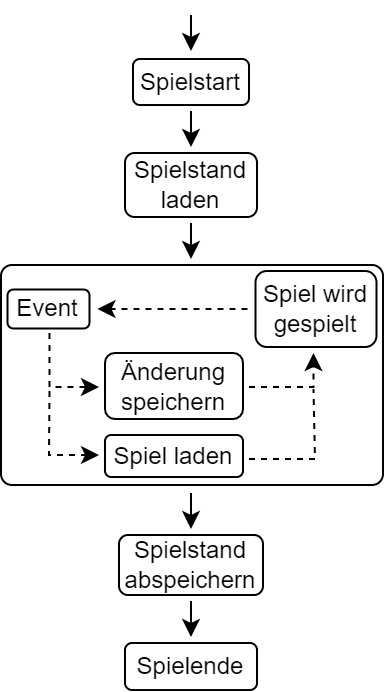
\includegraphics[width=0.36\textwidth]{images/Speichersystem.png}
    \caption{Phasen eines allgemeinen Speicher- und Ladesystems}
    \label{fig:speicherphasen}
\end{figure}

\iffalse
\begin{itemize}
    \item Je nach Speichersystem können die Events die in "Änderung speichern" behandelt werden in zwei Kategorien unterteilt werden:
    \begin{enumerate}
        \item Ein Spielobjekt wurde hinzugefügt/geändert
        \item Ein Spielobjekt wurde gelöscht
    \end{enumerate}
\end{itemize}
\fi
%--------------------------------------------------------------------------


%--------------------------------------------------------------------------
\subsection{Chunk-basiertes System}
Sei die Welt theoretisch unendlich, dann ist ein Chunk-System unter den sinnvollsten Aufteilungen der Daten für ein Speicher- und Ladesystem. In der Abbildung \ref{fig:chunkClass} ist zu sehen, aus welchen Attributen die Chunk-Klasse besteht. Jeder Chunk hat eine Identifikationsnummer, Position, Größe und Elemente. Die Position kann die Mitte des Chunks sein, oder ein Eckpunkt. Position und Größe sind dabei zwei- oder dreidimensionale Vektoren, je nachdem in welcher Dimension das Spiel gespielt wird. Der Typ der Elemente hängt von dem Chunk ab. Das ausgewählte Chunk-System hat für jeden zu speichernden Datentyp ein eigenes Chunk-Subsystem. Wenn es zu viele Datentypen gibt, ist es sinnvoller, in einem Chunk alle Spielobjekte gemeinsam zu speichern, egal welchen Datentyp diese haben. Optional ist es noch, die ParentID und ChildrenID zu speichern. Wenn für ein dynamisches Chunk-System entschieden wird, dann können die alten Chunks, die auf kleiner Chunks aufgeteilt wurden, erhalten bleiben. Damit dann eine Relation zwischen den alten Chunks und den neuen Chunks gibt, können diese mit einer Eltern-Kind-Relation verbunden werden. Jeder Eltern-Chunk hat vier Kinder-Chunk, wenn der Eltern-Chunk aufgeteilt wurde. Beim Vereinigen von Chunks können die Elemente dieser auch leichter an den Eltern-Chunk weitergegeben werden. Danach können die Kinder-Chunks gelöscht werden.

\begin{figure}[htp]
    \centering
    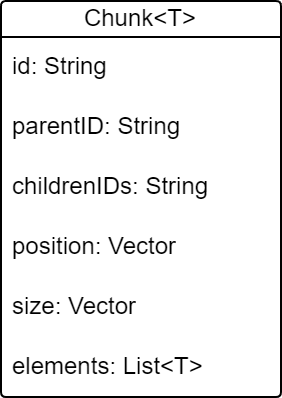
\includegraphics[width=0.28\textwidth]{images/Chunk.png}
    \caption{Chunk Klasse}
    \label{fig:chunkClass}
\end{figure}

In der Abbildung \ref{fig:chunkBasedSystem} ist ein Ablaufdiagramm zu dem ersten Ansatz eines Chunk-basierten Systems zu erkennen. Nach Spielstart werden zu Begin die Informationen der einzelnen Chunks geladen. Hiermit sind alle Informationen außer den Elementen eines Chunks gemeint, denn im nächsten Schritt sollen die Elemente der Chunks in der Nähe des Spielers geladen werden. Dafür werden die Positionen und Größen aller Chunks benötigt. Damit ein Lazy Loading stattfindet, werden mit diesem Ansatz nur die Elemente in der Nähe des Spielers geladen. In der Hauptphase des Spieles werden dann weiterhin die Chunk-Elemente der Chunks geladen, die in der Nähe des Spielers sind. Die Chunk-Veränderungen zu speichern, hängt bei dieser Strategie davon ab, ob die Chunks eine feste Größe haben oder nicht. Wird eine feste Chunkgröße gewählt, so muss der Chunkinhalt, also die Elemente eines Chunks, jedes Mal neu angepasst werden, wenn ein Objekt verändert, hinzugefügt oder gelöscht wurde.  Bei einer dynamischen Chunkgröße, wie in \ref{sssect:chunks} gezeigt, wird ähnlich bei Modifikation, Hinzufügung und Löschung von Spielobjekten gearbeitet, nur muss noch zusätzlich jedes Mal die Größe des Chunkinhaltes überprüft werden. Wenn ein Chunk zu viele Elemente hat, müssen diese auf neue, kleinere Chunks verteilt werden. Wenn ein Chunk zu wenig Elemente hat, müssen diese wieder in dem Eltern-Chunk gespeichert werden und dessen Kind-Chunks müssen im Speicher wieder herausgenommen werden.

\begin{figure}[htp]
    \centering
    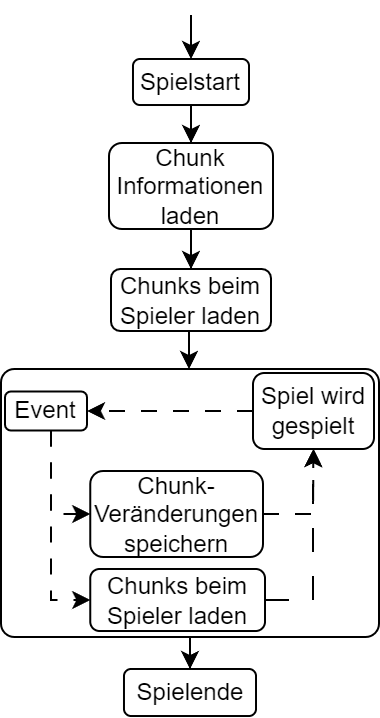
\includegraphics[width=0.36\textwidth]{images/Chunkbasiert.png}
    \caption{Chunk-basiertes System}
    \label{fig:chunkBasedSystem}
\end{figure}

Eine Erweiterung des Chunk-basierten Systems wäre das Hinzufügen einer Change-Datei, wo alle Veränderungen der Spielwelt abgespeichert werden, wie in \ref{ssect:deltasave} gezeigt. Die Veränderungen können in einer Liste gespeichert werden, als Objekte der Klasse der Abbildung \ref{fig:changesClass}. Diese Klasse besteht aus einem ID-, Event- und Objekt-Attribut. Das Event kann kennzeichnen, ob ein Spielobjekt hinzugefügt, verändert oder gelöscht wurde. Je nach Event sieht dann das Objekt auch anders aus. Wenn ein Spielobjekt verändert wurde, reicht es dort die ID des Objekts und die veränderten Attribute mit deren Werten zu speichern. Falls ein Spielobjekt gelöscht wurde, reicht es hier, die ID des gelöschten Objektes anzugeben. Für den Fall, dass ein Spielobjekt neu hinzugefügt wurde, kann hier das komplette Spielobjekt übergeben werden. Zu den veränderten Daten müssen auch die Chunks betrachtet werden. Falls ein Spielobjekt zu einem anderen Chunk verschoben wurde, muss dies der Change-Datei übergeben werden. Wenn ein dynamisches Chunk-System verwendet wird, muss außerdem noch in der Change-Datei gespeichert werden, wenn ein Chunk erstellt oder gelöscht wurde. Durch diese Strategie werden die Schreib- und Leseprozesse in dem lokalen Speicher stark reduziert, da während der Laufzeit des Spieles nur die Veränderungen gespeichert werden und kein Chunkinhalt neu angepasst werden muss.

\begin{figure}[htp]
    \centering
    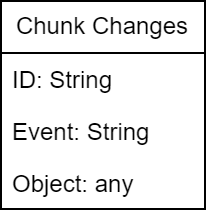
\includegraphics[width=0.25\textwidth]{images/Changes.png}
    \caption{Speichern von Veränderungen}
    \label{fig:changesClass}
\end{figure}

In der Abbildung \ref{fig:altchunkBasedSystem} ist das Ablaufdiagramm des Chunk-basierten Speicher- und Ladesystems mit Change-Datei zu sehen. Wie zu sehen gibt es einige Parallelen zu dem System aus der Abbildung \ref{fig:chunkBasedSystem}. Ein paar Phasen sind etwas anders oder neu. Zu Beginn müssen die Veränderungen des letzten Spielstandes in die ganzen lokalen Daten der Chunkinhalte übertragen werden. Dafür muss die Change-Datei von oben nach unten abgearbeitet werden, da in den ersten Zeilen die ältesten Veränderungen sind. Zum Beispiel kann es sein, dass zweimal die Position eines Spielobjektes verändert wurde. Die ältere Position wurde zuerst in die Change-Datei gespeichert und wird dann durch das Abarbeiten von oben nach unten durch die neue Position überschrieben. Danach kann die Change-Datei wieder geleert werden, um wieder die neuen Veränderungen sammeln zu können. Eine weitere Anpassung ist das Speichern der Veränderungen. Hier werden nicht die lokalen Chunk-Daten aktualisiert, sondern stattdessen die Veränderungen der Change-Datei übergeben. Der Rest läuft genau gleich ab, wie bei der vorherigen Chunk-basierten Strategie.

\begin{figure}[htp]
    \centering
    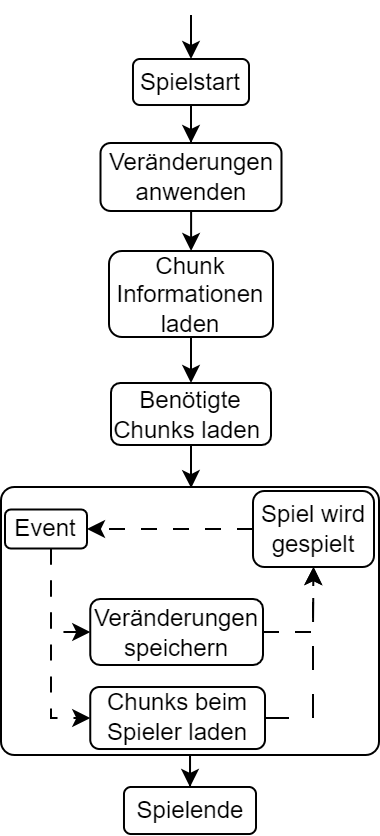
\includegraphics[width=0.36\textwidth]{images/Chunkbasiert2.png}
    \caption{Alternative zu dem Chunk-basierten System}
    \label{fig:altchunkBasedSystem}
\end{figure}
%--------------------------------------------------------------------------


%--------------------------------------------------------------------------
\subsection{Auswertung}
Auswertung der Strategien mit Daten/einfaches Spielkonzept mit Java und \ac{json} testen:
\begin{itemize}
    \item Spieler (HP, LVL, Ausrüstung, Position, Rotation, ...)
    \item Gegner (HP, LVL, Ausrüstung, Position, Rotation, ...)
    \item Ausrüstung (Beschreibung/ID, Verteidigung, Angriff)
    \item Hindernisse (Beschreibung/ID, Position, Rotation)
    \item Items (Beschreibung/ID, Position, Rotation)
\end{itemize}

\begin{figure}[htp]
    \centering
    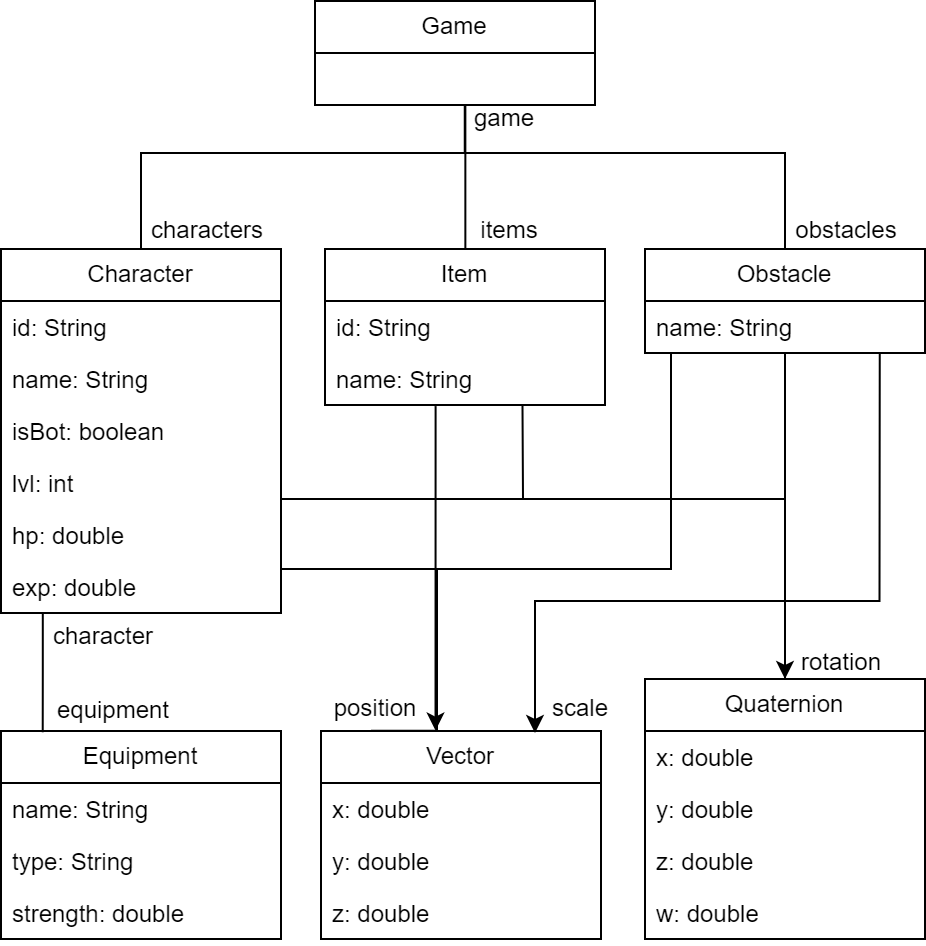
\includegraphics[width=0.8\textwidth]{images/Klassendiagramm.png}
    \caption{Klassendiagramm des Spieles}
    \label{fig:classDia}
\end{figure}

Klassendiagramm zeigen, um Daten des Spieles zu visualisieren. Testen der Effizienz mit JMH (Erklären was JMH ist und warum das gut dafür ist)

Zu beachtende Faktoren:
\begin{itemize}
    \item Chunk size
    \item Veränderungen
\end{itemize}